\section*{3. Compute, Runtime, And Public Calibration}

The project used both the MacBook and the MBZUAI HPC lab, but not for the same kind of work. Short MPS-supported experiments and compact meta models were comfortable on the Mac. Wider classifier families, cross-validated neural runs, and the professor lane made more sense on HPC, where the logs explicitly show workstations such as \texttt{ws-l5-031} and \texttt{ws-l5-032}.

\begin{figure}[H]
    \centering
    \begin{subfigure}[t]{0.58\linewidth}
        \centering
        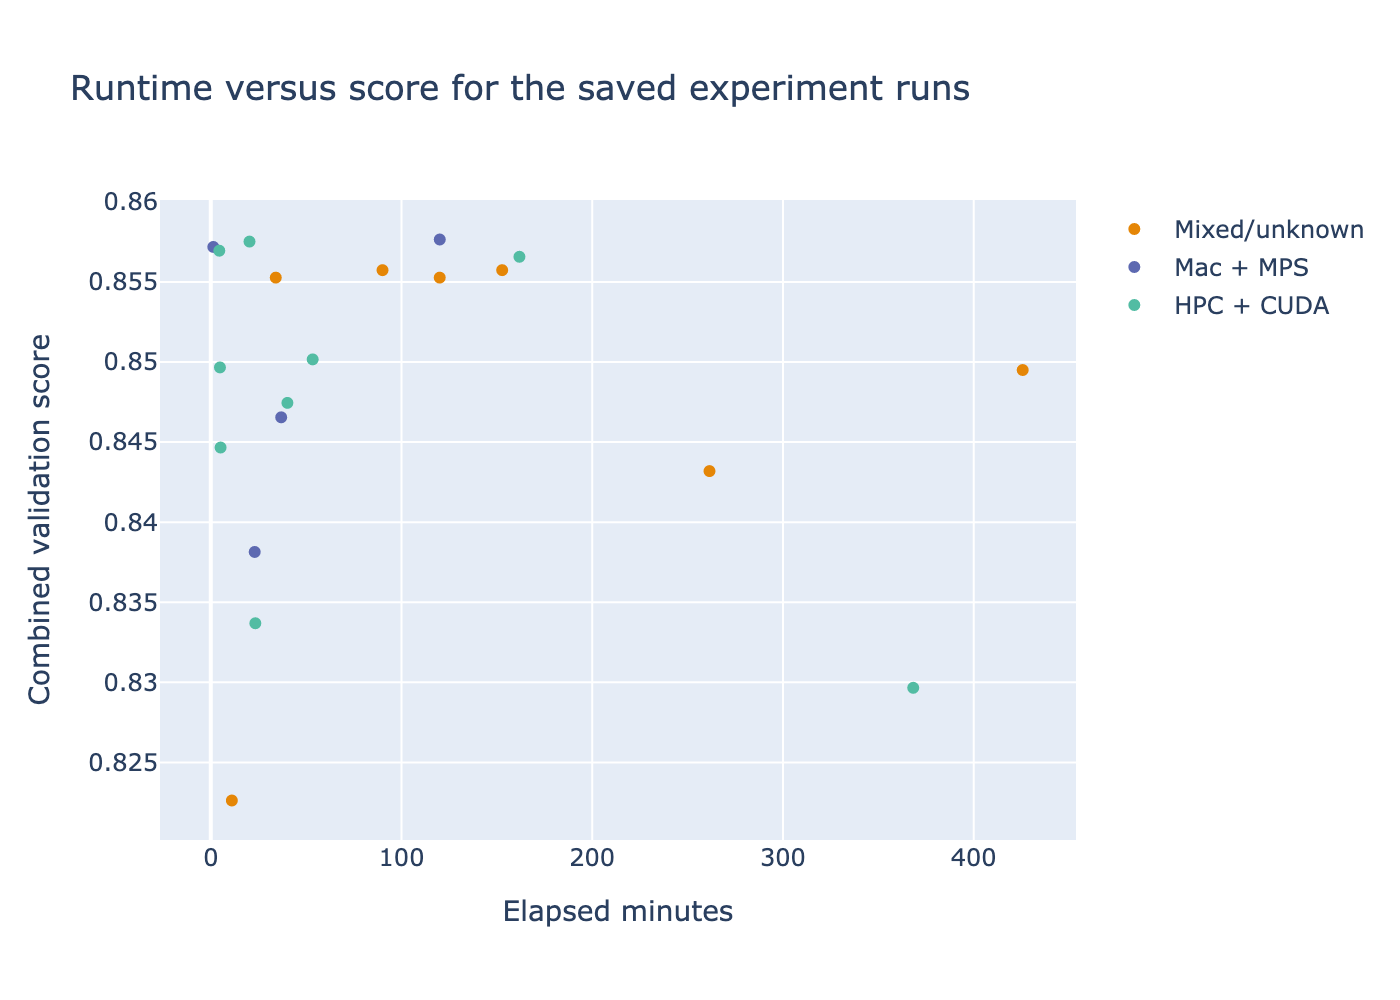
\includegraphics[width=\linewidth]{figures/methods_runtime_tradeoff.png}
        \caption{Runtime versus score for the saved runs.}
    \end{subfigure}\hfill
    \begin{subfigure}[t]{0.38\linewidth}
        \centering
        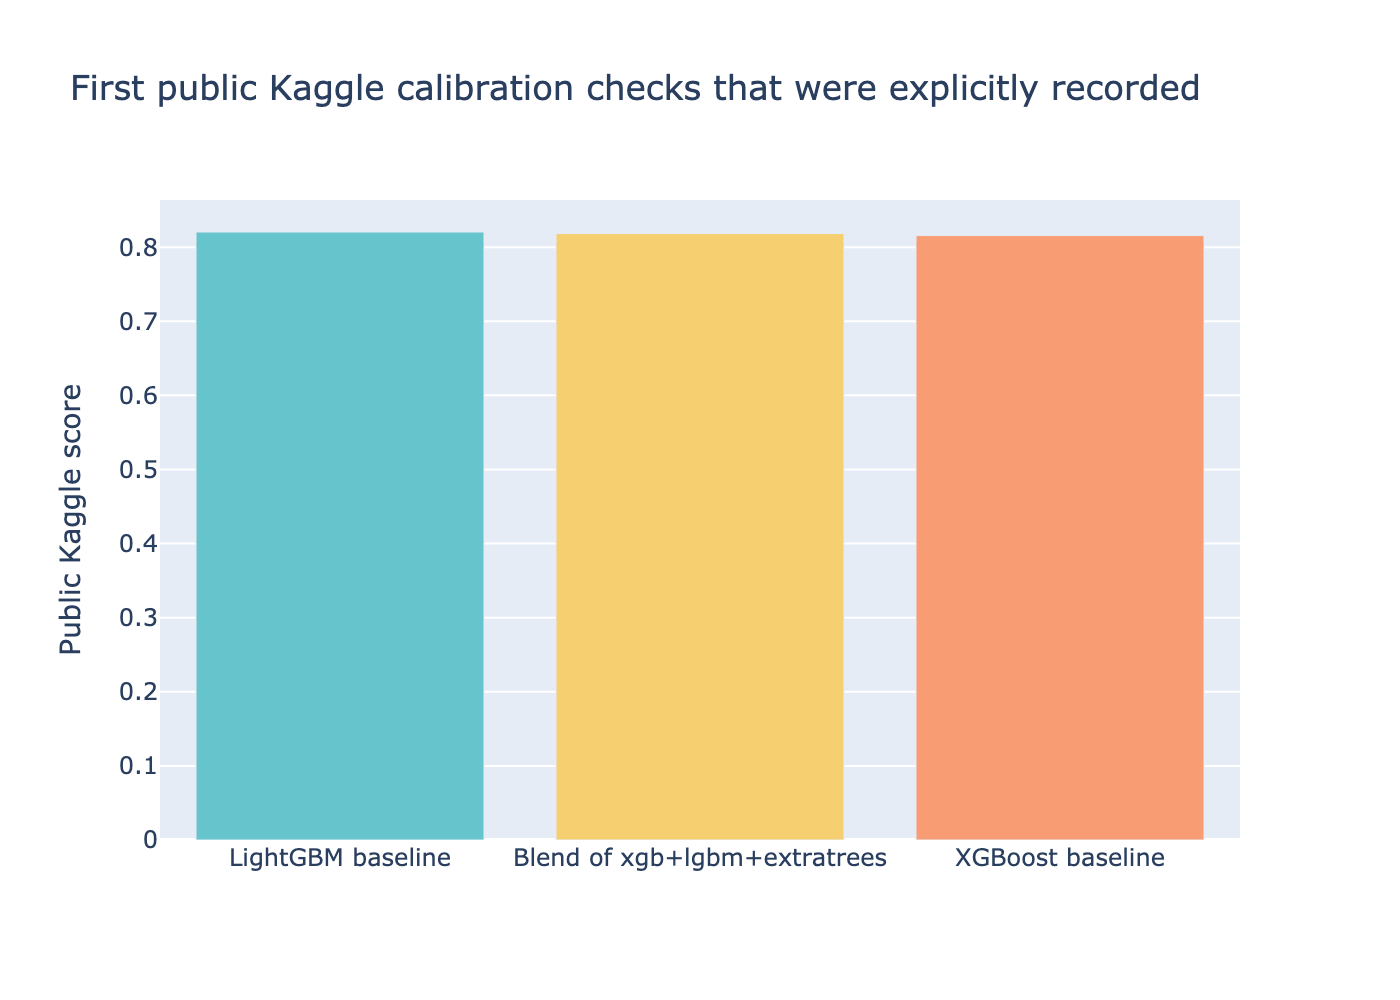
\includegraphics[width=\linewidth]{figures/methods_public_checks.png}
        \caption{The early public Kaggle checks that were explicitly recorded.}
    \end{subfigure}
    \caption{The project needed both local speed and cluster muscle. Public Kaggle checks were used sparingly, mostly to calibrate the local metric rather than replace it.}
\end{figure}

\rowcolors{2}{coolbg}{white}
\begin{table}[H]
    \centering
    \small
    \begin{tabularx}{\linewidth}{>{\bfseries}p{0.30\linewidth} >{\centering\arraybackslash}p{0.18\linewidth} >{\centering\arraybackslash}p{0.16\linewidth} X}
        \rowcolor{ink!12}
        Run & Score & Minutes & Compute note \\
        \texttt{mlp\_meta\_stack\_v1} & 0.857181 & 1.33 & Tiny Mac-side meta model; very cheap and surprisingly effective. \\
        \texttt{mlp\_weighted\_blend\_v1} & 0.857645 & 120.06 & Mac/MPS blend search; best local result that survived in the saved artifacts. \\
        \texttt{classifier\_holdout\_blend\_v2} & 0.857517 & 20.31 & HPC/CUDA run; strong late-stage competitor, especially on the classification side. \\
        \texttt{approach\_professor\_target\_stats} & 0.856566 & 161.83 & HPC refresh of the target-stats branch after the professor suggestions. \\
        \texttt{tree\_teacher\_classifier\_bagging\_v2} & 0.829660 & 368.29 & Expensive and technically interesting, but not a practical winner on the project metric. \\
    \end{tabularx}
    \caption{A few runtime snapshots show the real trade-off: some of the best ideas were cheap, while some of the most expensive ones were mainly educational.}
\end{table}

The public leaderboard was helpful, but only in small doses. The first Kaggle calibration on March 20 showed that the local ranking was useful: LightGBM was best publicly among the first three, the blend was close behind, and XGBoost trailed slightly. That was enough to justify keeping Kaggle as a checkpoint rather than turning the whole project into a submission lottery.

Later public scores were not kept with the same level of detail in the retained artifacts, so the second half of the project had to lean mostly on saved validation tables and training logs.
